% author: Simon Bachmann

\section{Problem Statement and Motivation}
Today's event ticketing industry has a fundamental flaw. The existing systems for distributing tickets are open for a lot of arbitrage during the time the ticket is sold until the event happens. This means that besides the primary seller of the tickets (e.g. event organizer) intermediaries make a profit by buying, reselling and counterfeiting tickets. 

Figure \ref{fig:ticketing-industry-landscape} gives an overview of today's event ticketing landscape with its most important actors and how they interact with each other. The secondary market is where the major issue lies and ticket scalper can scoop profits.

\begin{figure}[H]
    \centering
    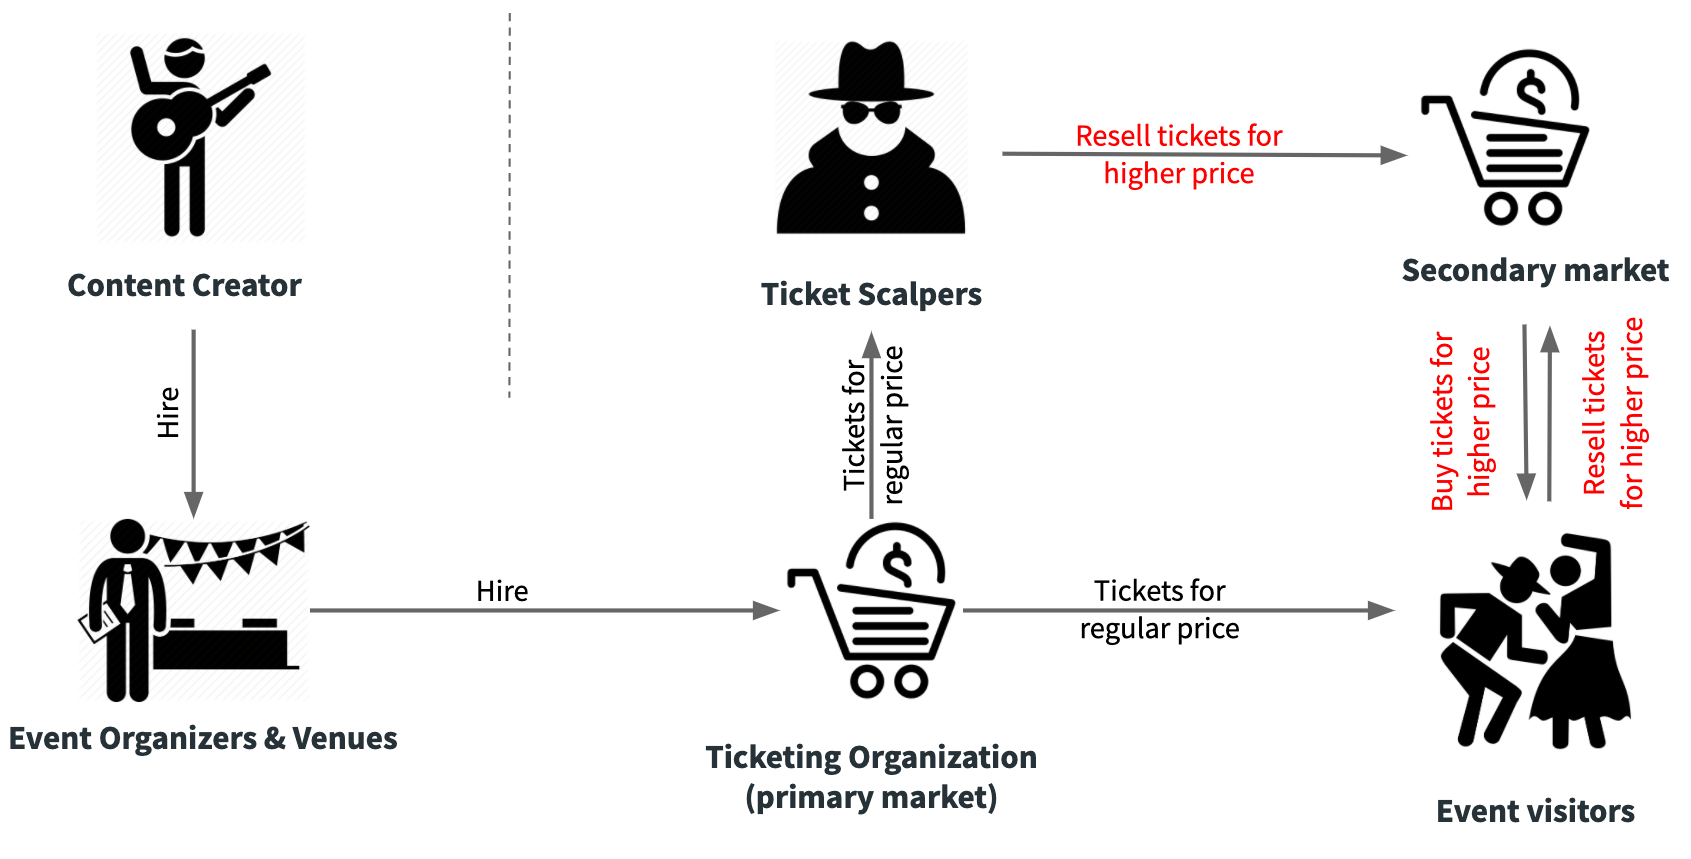
\includegraphics[width=16cm]{figures/ticketing-industry-landscape.png}
    \caption{Actors in the ticketing industry}
    \label{fig:ticketing-industry-landscape}
\end{figure}

\subsection{Motivation}
- authenticity and tractability of tickets
- open standardised backend. multiple front end can connect to it and benefit from the network effect
- fair and transparent a fee structure of affiliate network

\subsection{Distributed Ledger Technology (DLT)}
Event ticketing companies already issue event tickets digitally. The question arises why it makes sense to use a blockchain where transactions are slow, expensive and for many users difficult to interact with. 

Building an open standard tokenized goods that rely on a regulated aftermarket on a blockchain has several advantages.

\begin{itemize}
	\item Because the tickets are stored on a publicly accessible database, anybody can verify whether a ticket is real without the need of a trusted third party.
	\item Less intermediaries such as payment processors are needed because digital currencies are available in the blockchain ecosystem. 
	\item A standard for digital tickets enables the interoperability between different products/application. Similar to others standards emerging in the blockchain ecosystem, it allows different applications to plug into the system and benefit from network effects. Decoupling the data layer (e.g. blockchain) from the user interaction layer (e.g. GUI) results in more competition for frontend applications an thus often better products. Comparing such an approach with today's landscape, one can think of having one shared database among companies such as Starticket and Ticketcorner (primary market), Ebay and Ricardo (secondary market). A reward system included in the ticket standard incentives primary markets as well as secondary markets to participate in the systems. 
	\item The end user must only check on his favourite ticketing platform if tickets are available since all platforms connect to the same backend.
	\item Stakeholders such as affiliate and GUI providers 
\end{itemize}


\begin{figure}[H]
    \centering
    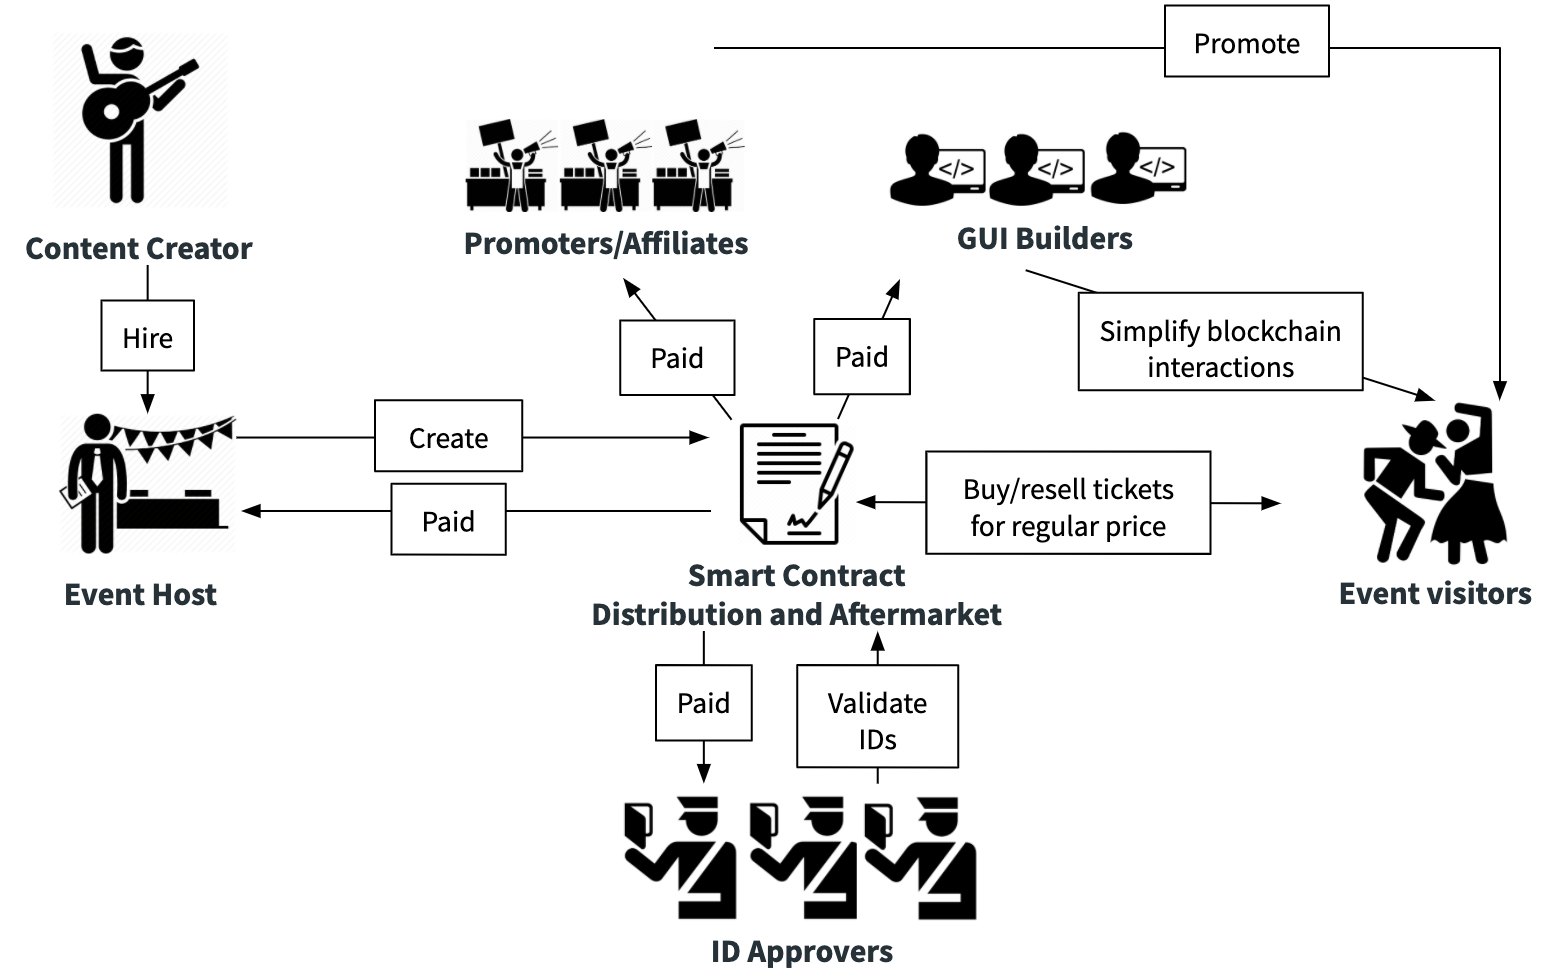
\includegraphics[width=16cm]{figures/dlt-based-landscape.png}
    \caption{DLT-based architecture}
    \label{fig:dlt-based-landscape}
\end{figure}

